% !TEX program = xelatex
% ============================================================================
%  POSN Computer Qualification — Functions Slide Deck
%  Topic: ความสัมพันธ์และฟังก์ชัน (Relations and Functions)
% ============================================================================

\documentclass[11pt, aspectratio=169]{beamer}

% --- Load shared preamble ---
% ============================================================================
%  POSN Computer Qualification — Shared Beamer Preamble
%  Used by all topic slide decks. Compile with XeLaTeX.
% ============================================================================

% ---------- Thai language & font ----------
\usepackage{iftex}
\usepackage{fontspec}

% XeTeX-specific: enable Thai line breaking
\ifXeTeX
  \XeTeXlinebreaklocale{th}
\fi
% Noto Sans Thai — body text (clean modern sans-serif, handles all Thai)
\setmainfont{Noto Sans Thai}[
  UprightFont = Noto Sans Thai Light,
  BoldFont    = Noto Sans Thai Medium,
  Scale       = 0.9
]
\setsansfont{Noto Sans Thai}[
  UprightFont = Noto Sans Thai Light,
  BoldFont    = Noto Sans Thai Medium,
  Scale       = 0.9
]

% Noto Sans Thai — clean modern sans-serif for structural elements
\newfontfamily\headingfont{Noto Sans Thai}[
  UprightFont = Noto Sans Thai Medium,
  BoldFont    = Noto Sans Thai Bold,
  Scale       = 0.9
]

% --- Heading font for structural elements ---
\setbeamerfont{title}{family=\headingfont, series=\bfseries, size=\huge}
\setbeamerfont{subtitle}{family=\headingfont, series=\mdseries}
\setbeamerfont{author}{family=\headingfont, series=\mdseries}

% --- Custom Title Page ---
\defbeamertemplate{title page}{custom}[1][]{%
  \centering
  \vspace*{2cm}
  % Title — in white
  {\usebeamerfont{title}\color{white}\inserttitle\par}
  \vspace{0.6cm}
  % Subtitle — in white
  {\usebeamerfont{subtitle}\color{white}\insertsubtitle\par}
  \vspace{2.5cm}
  % Author — blue filled rounded box, white text
  \begin{center}
    \begin{tcolorbox}[arc=3mm, colback=boxBlue, colframe=boxBlue!80,
                      width=0.42\textwidth, halign=center,
                      left=1.5em, right=1.5em, top=0.8em, bottom=0.8em,
                      boxrule=1.5pt, coltext=white]
      \usebeamerfont{author}\insertauthor
    \end{tcolorbox}
  \end{center}
}
\setbeamertemplate{title page}[custom]
\setbeamerfont{frametitle}{family=\headingfont, series=\bfseries}
\setbeamerfont{section in toc}{family=\headingfont}
\setbeamerfont{page number in head/foot}{family=\headingfont}
\setbeamerfont{section title}{family=\headingfont, series=\bfseries}
\setbeamerfont{subsection title}{family=\headingfont}

% Monospace font (for code/verbatim)
\setmonofont{Latin Modern Mono}[Scale=0.9]

% ---------- Math ----------
\usepackage{amsmath, amssymb}

% ---------- Graphics ----------
\usepackage{graphicx}
\usepackage{tikz}

% ---------- String parsing (for section headers) ----------
\usepackage{xstring}

% ---------- Colored boxes ----------
\usepackage[skins, breakable, xparse]{tcolorbox}
% Note: we do NOT load the 'most' option — it predefines example/solution environments
% that would conflict with our custom boxes.

% --- Color definitions ---
\definecolor{boxBlue}{RGB}{41, 128, 185}
\definecolor{boxGreen}{RGB}{39, 174, 96}
\definecolor{boxOrange}{RGB}{230, 126, 34}
\definecolor{boxPurple}{RGB}{142, 68, 173}
\definecolor{boxBlueBg}{RGB}{235, 245, 255}
\definecolor{boxGreenBg}{RGB}{235, 255, 240}
\definecolor{boxOrangeBg}{RGB}{255, 245, 235}
\definecolor{boxPurpleBg}{RGB}{248, 240, 255}

% --- Explanation box (blue) — for definitions, concepts, notes ---
\newtcolorbox{explanation}[1][]{
  enhanced,
  breakable,
  arc         = 2mm,
  colback     = boxBlueBg,
  colframe    = boxBlue!50,
  title       = #1,
  fonttitle   = \bfseries\color{white},
  coltitle    = white,
  colbacktitle= boxBlue,
  attach boxed title to top left = {yshift=-2mm, xshift=2mm},
  boxed title style = {arc=2mm, size=small},
  before skip = 8pt,
  after skip  = 8pt
}

% --- Example box (green) — for worked examples ---
\newtcolorbox{exambox}[1][]{
  enhanced,
  breakable,
  arc         = 2mm,
  colback     = boxGreenBg,
  colframe    = boxGreen!50,
  title       = #1,
  fonttitle   = \bfseries\color{white},
  coltitle    = white,
  colbacktitle= boxGreen,
  attach boxed title to top left = {yshift=-2mm, xshift=2mm},
  boxed title style = {arc=2mm, size=small},
  before skip = 8pt,
  after skip  = 8pt
}

% --- Solution box (orange) — for solutions and answers ---
\newtcolorbox{solbox}[1][]{
  enhanced,
  breakable,
  arc         = 2mm,
  colback     = boxOrangeBg,
  colframe    = boxOrange!50,
  title       = #1,
  fonttitle   = \bfseries\color{white},
  coltitle    = white,
  colbacktitle= boxOrange,
  attach boxed title to top left = {yshift=-2mm, xshift=2mm},
  boxed title style = {arc=2mm, size=small},
  before skip = 8pt,
  after skip  = 8pt
}

% --- Intuition box (purple) — for plain-language explanations, analogies ---
\newtcolorbox{intuition}[1][]{
  enhanced,
  breakable,
  arc         = 2mm,
  colback     = boxPurpleBg,
  colframe    = boxPurple!50,
  title       = #1,
  fonttitle   = \bfseries\color{white},
  coltitle    = white,
  colbacktitle= boxPurple,
  attach boxed title to top left = {yshift=-2mm, xshift=2mm},
  boxed title style = {arc=2mm, size=small},
  before skip = 8pt,
  after skip  = 8pt
}

% ---------- Beamer theme ----------
\usetheme{Madrid}
\usecolortheme{default}

% --- Custom beamer colors (blue accent matching explanation boxes) ---
\setbeamercolor{structure}{fg=boxBlue}
\setbeamercolor{palette primary}{fg=white, bg=boxBlue}
\setbeamercolor{palette secondary}{fg=white, bg=boxBlue!80}
\setbeamercolor{palette tertiary}{fg=white, bg=boxBlue!60}
\setbeamercolor{block title}{fg=white, bg=boxBlue}
\setbeamercolor{block body}{fg=black, bg=boxBlueBg}

% Remove navigation symbols for clean look
\setbeamertemplate{navigation symbols}{}

% Note: Frame title prefix removed — \addtobeamertemplate conflicts with beamer internals

% --- Outline (Table of Contents) styling ---
\setbeamerfont{section in toc}{family=\headingfont, series=\mdseries}
\setbeamerfont{subsection in toc}{family=\headingfont, series=\mdseries}
\setbeamertemplate{section in toc}{%
  \leavevmode\leftskip=1.5em
  \textcolor{boxBlue}{\textbf{\large\inserttocsectionnumber.}}%
  \quad\inserttocsection\par
  \vspace{0.2em}
}
\setbeamertemplate{subsection in toc}{%
  \leavevmode\leftskip=4em
  \textcolor{boxBlue!60}{\small$\bullet$}%
  \quad\inserttocsubsection\par
  \vspace{0.1em}
}

% Section header slides — Thai in white, English in smaller light blue below
\AtBeginSection{
  \begin{frame}[plain]{}
    \vspace*{2cm}
    \begin{beamercolorbox}[sep=12pt, center, rounded=true, shadow=true]{palette primary}
      \IfSubStr{\secname}{(}{%
        \StrBefore{\secname}{(}[\sectionthai]%
        \StrBetween[1,1]{\secname}{(}{)}[\sectioneng]%
        \begin{tabular}{@{}c@{}}
          {\usebeamerfont{title}\sectionthai} \\[0.2em]
          {\usebeamerfont{subtitle}\color{boxBlue!60}\sectioneng}
        \end{tabular}%
      }{%
        {\usebeamerfont{title}\secname\par}%
      }
    \end{beamercolorbox}
    \vfill
  \end{frame}
}

% Subsection header slides — smaller, centered
\AtBeginSubsection{
  \begin{frame}[plain]{}
    \vfill
    \centering
    {\usebeamerfont{section title}\insertsubsectionhead\par}
    \vfill
  \end{frame}
}

% Minimal footer: page number only, right-aligned
\setbeamertemplate{footline}{
  \hfill\usebeamerfont{page number in head/foot}\insertframenumber{} / \inserttotalframenumber\hspace*{1em}\vspace*{0.5ex}
}

% ---------- Spacing & readability ----------
\linespread{1.2}

% ---------- Useful commands ----------

% Highlight important text in blue
\newcommand{\highlight}[1]{\textcolor{boxBlue}{\textbf{#1}}}

% Math set notation helpers
\newcommand{\R}{\mathbb{R}}
\newcommand{\N}{\mathbb{N}}
\newcommand{\Z}{\mathbb{Z}}
\newcommand{\Q}{\mathbb{Q}}

% ============================================================================
%  End of preamble
% ============================================================================


% --- Document info ---
\title[ความสัมพันธ์และฟังก์ชัน]{\textcolor{white}{ความสัมพันธ์และฟังก์ชัน} \\ \textcolor{boxBlue!60}{(Relations and Functions)}}
\subtitle{ความสัมพันธ์ • ฟังก์ชัน • ประเภทของฟังก์ชัน • คุณสมบัติของความสัมพันธ์ }
\author[None Wanitchollakit]{None W. (Yuan)}
\date{}

\begin{document}

% ===========================================================================
%  TITLE SLIDE
% ===========================================================================
\begin{frame}[plain]
  \titlepage
\end{frame}

% ===========================================================================
%  OUTLINE
% ===========================================================================
\begin{frame}{สารบัญ (Outline)}
  \tableofcontents
\end{frame}

% ===========================================================================
%  SECTION: บทนำ — ความสัมพันธ์ (Relations)
% ===========================================================================
\section{ความสัมพันธ์ (Relations)}

\begin{frame}{ความสัมพันธ์คืออะไร?}
  \begin{explanation}[นิยาม: ความสัมพันธ์ (Relation)]
    ให้ $A$ และ $B$ เป็นเซตใด ๆ \textbf{ความสัมพันธ์} $r$ จาก $A$ ไปยัง $B$
    คือ \highlight{เซตย่อยของผลคูณคาร์ทีเซียน} $A \times B$

    \medskip
    นั่นคือ $r \subseteq A \times B$

    \medskip
    ถ้า $(a, b) \in r$ เรากล่าวว่า $a$ \textbf{มีความสัมพันธ์} $r$ กับ $b$
    และเขียนแทนด้วย $a \; r \; b$
  \end{explanation}

  \begin{itemize}
    \item $A$ เรียกว่า \highlight{เซตตั้งต้น} (domain set)
    \item $B$ เรียกว่า \highlight{เซตปลายทาง} (codomain set)
  \end{itemize}

  \begin{exambox}[ตัวอย่าง]
    ความสัมพันธ์เหมือนกับการจับคู่ เช่น $r=\left\{(1,2),(1,-2),(3, 9)\right\} $ เป็นต้น
  \end{exambox}
\end{frame}

\begin{frame}{ผลคูณคาร์ทีเซียน (Cartesian Product)}
  \begin{explanation}[นิยาม: ผลคูณคาร์ทีเซียน]
    \textbf{ผลคูณคาร์ทีเซียน} ของเซต $A$ และ $B$ คือเซตของคู่อันดับ $(a, b)$ ทั้งหมด
    โดยที่ $a \in A$ และ $b \in B$

    \medskip
    $A \times B = \{(a, b) \mid a \in A \text{ และ } b \in B\}$
  \end{explanation}

  \begin{exambox}[ตัวอย่าง]
    ให้ $A = \{1, 2\}$ และ $B = \{a, b, c\}$

    \medskip
    $A \times B = \{(1,a), (1,b), (1,c), (2,a), (2,b), (2,c)\}$

    \medskip
    $|A \times B| = |A| \times |B| = 2 \times 3 = 6$
  \end{exambox}
\end{frame}

\begin{frame}{โดเมนและเรนจ์ของความสัมพันธ์}
  \begin{explanation}[นิยาม]
    ให้ $r$ เป็นความสัมพันธ์จาก $A$ ไปยัง $B$

    \medskip
    \textbf{โดเมน} (Domain) ของ $r$:
    \quad $D_r = \{a \in A \mid \text{มี } b \in B \text{ ที่ } (a,b) \in r\}$

    \medskip
    \textbf{เรนจ์} (Range) ของ $r$:
    \quad $R_r = \{b \in B \mid \text{มี } a \in A \text{ ที่ } (a,b) \in r\}$
  \end{explanation}

  \begin{itemize}
    \item โดเมน $\subseteq A$ — เฉพาะสมาชิกของ $A$ ที่ถูกใช้
    \item เรนจ์ $\subseteq B$ — เฉพาะสมาชิกของ $B$ ที่ถูกใช้
  \end{itemize}

  \begin{intuition}[สังเกต]
    ง่าย ๆ โดเมน คือ ตัวหน้าของคู่ ($a$) เป็นอะไรได้บ้าง เรนจ์ คือ ตัวหน้าของคู่ ($b$) เป็นอะไรได้บ้าง
  \end{intuition}
\end{frame}

\begin{frame}{ตัวอย่าง: การหาโดเมนและเรนจ์}
  \begin{exambox}[โจทย์]
    กำหนด $r = \{(x, y) \mid y = x^2,\; x \in \{-2, -1, 0, 1, 2\}\}$
    จงหา $D_r$ และ $R_r$
  \end{exambox}

  \begin{solbox}[วิธีทำ]
    แทนค่า $x$ แต่ละตัวลงในสมการ $y = x^2$:
    \begin{align*}
      x = -2 &\Rightarrow y = 4 \\
      x = -1 &\Rightarrow y = 1 \\
      x = 0  &\Rightarrow y = 0 \\
      x = 1  &\Rightarrow y = 1 \\
      x = 2  &\Rightarrow y = 4
    \end{align*}
  \end{solbox}
\end{frame}

\begin{frame}{ตัวอย่าง: การหาโดเมนและเรนจ์ (ต่อ)}
  \begin{solbox}[วิธีทำ (ต่อ)]
    จะได้ $r = \{(-2,4), (-1,1), (0,0), (1,1), (2,4)\}$ \newline
    รวบรวมผลลัพธ์:

    $D_r = \{-2, -1, 0, 1, 2\}$ \quad (ค่า $x$ ทั้งหมดที่โจทย์กำหนด)

    $R_r = \{0, 1, 4\}$ \quad (ค่า $y$ ที่เกิดขึ้น โดยไม่นับซํ้า)
  \end{solbox}

  \medskip
  \begin{intuition}[สังเกต]
    โดเมนคือค่า $x$ ที่ใส่เข้าไป เรนจ์คือค่า $y$ ที่ได้ออกมา
  \end{intuition}
\end{frame}

\begin{frame}{ตัวอย่าง: ข้อสอบจริง}
  \begin{exambox}[โจทย์ปี 68 ข้อ 10]
    กำหนด $A=\{1,2,3\}, B=\{4,5\}$ และความสัมพันธ์ $r$ จากเซต $A$ ไปยังเซต $B$ โดย $r=\{(a,b)\in A\times B\mid a+b$ เป็นจำนวนคี่ $\}$ ข้อใดเป็นจริง \newline
    [ข. $r$ มีสมาชิก 6 คู่อันดับ]
    [ง. $r$ ไม่มีสมาชิกเลย]
  \end{exambox}

  \begin{solbox}[วิธีทำ]
    $A\times B = \{(1,4), (1,5), (2,4), (2,5), (3,4), (3,5)\}$ \newline
    ในจำนวนนี้ที่มีผลรวม $(a+b)$ เป็นจำนวนคี่ ได้แก่ $(1,4), (2,5), (3,4)$ \newline
    ดังนั้น $r = \{(1,4), (2,5), (3,4)\}$ \newline
    \textbf{ข. และ ง. ผิด เพราะ $r$ มีสมาชิก 3 คู่อันดับ}
  \end{solbox}
\end{frame}

% ===========================================================================
%  SECTION: ฟังก์ชัน (Functions)
% ===========================================================================
\section{ฟังก์ชัน (Functions)}

\begin{frame}{ฟังก์ชันคืออะไร?}
  \begin{explanation}[นิยาม: ฟังก์ชัน (Function)]
    \textbf{ฟังก์ชัน} คือความสัมพันธ์ที่สมาชิกแต่ละตัวในโดเมน
    \highlight{จับคู่กับสมาชิกในเรนจ์เพียงตัวเดียวเท่านั้น}

    \medskip
    นั่นคือ ถ้า $(a, b_1) \in f$ และ $(a, b_2) \in f$ แล้ว $b_1 = b_2$
  \end{explanation}

  \begin{itemize}
    \item ฟังก์ชันเป็น \highlight{ความสัมพันธ์ชนิดพิเศษ}
    \item ทุกฟังก์ชันเป็นความสัมพันธ์ แต่ไม่ทุกความสัมพันธ์เป็นฟังก์ชัน
    \item เขียนแทนด้วย $f: A \to B$ หมายถึง $f$ เป็นฟังก์ชันจาก $A$ ไป $B$
  \end{itemize}

  \begin{intuition}[สังเกต]
    ง่าย ๆ ฟังก์ชัน คือ ความสัมพันธ์ที่จาก $x$ จับคู่ได้กับ $y$ ตัวเดียว เช่น $r = \left\{(x,y) \mid x = \left\lvert y\right\rvert \right\} $ ไม่ใช่ฟังก์ชัน เพราะ 1 มีความสัมพันธ์ $r$ กับทั้ง 1 และ -1
  \end{intuition}
\end{frame}

\begin{frame}{การทดสอบว่าเป็นฟังก์ชันหรือไม่}
  \begin{explanation}[การทดสอบแนวดิ่ง (Vertical Line Test)]
    กราฟจะเป็นกราฟของฟังก์ชัน ก็ต่อเมื่อ
    \highlight{เส้นตรงแนวดิ่งทุกเส้นตัดกราฟได้ไม่เกิน 1 จุด}
  \end{explanation}

  \begin{columns}[T]
    \column{0.45\textwidth}
      \centering
      \textbf{เป็นฟังก์ชัน} \\[1em]
      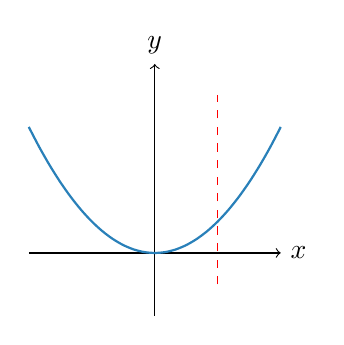
\begin{tikzpicture}[scale=0.8]
        \draw[->] (-2,0) -- (2,0) node[right] {$x$};
        \draw[->] (0,-1) -- (0,3) node[above] {$y$};
        \draw[domain=-2:2, smooth, thick, boxBlue] plot (\x, {0.5*\x*\x});
        \draw[dashed, red] (1, -0.5) -- (1, 2.5);
      \end{tikzpicture}
      \par เส้นแนวดิ่งตัดกราฟ 1 จุด $\checkmark$

    \column{0.45\textwidth}
      \centering
      \textbf{ไม่เป็นฟังก์ชัน} \\[1em]
      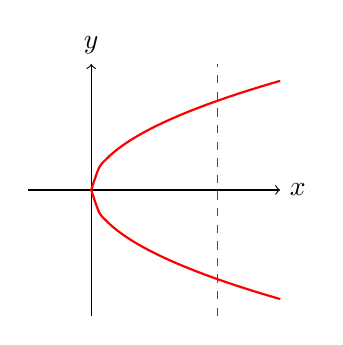
\begin{tikzpicture}[scale=0.8]
        \draw[->] (-1,0) -- (3,0) node[right] {$x$};
        \draw[->] (0,-2) -- (0,2) node[above] {$y$};
        \draw[domain=0:3, smooth, thick, red] plot (\x, {sqrt(\x)});
        \draw[domain=0:3, smooth, thick, red] plot (\x, {-sqrt(\x)});
        \draw[dashed, red] (2, -2) -- (2, 2);
      \end{tikzpicture}
      \par เส้นแนวดิ่งตัดกราฟ 2 จุด $\times$
  \end{columns}
\end{frame}

\begin{frame}{ตัวอย่าง: ข้อสอบจริง}
  \begin{exambox}[โจทย์ปี 68 ข้อ 10]
    กำหนด $A=\{1,2,3\}, B=\{4,5\}$ และความสัมพันธ์ $r$ จากเซต $A$ ไปยังเซต $B$ โดย $r=\{(a,b)\in A\times B\mid a+b$ เป็นจำนวนคี่ $\}$ ข้อใดเป็นจริง \newline
    [ก. $r$ เป็นฟังก์ชัน]
  \end{exambox}

  \begin{solbox}[วิธีทำ]
    จาก $r = \{(1,4), (2,5), (3,4)\}$ \newline
    \textbf{ก. ถูก เพราะ ความสัมพันธ์ที่สมาชิกแต่ละตัวในโดเมน $\{1,2,3\}$ จับคู่กับสมาชิกในเรนจ์เพียงตัวเดียวเท่านั้น}
  \end{solbox}
\end{frame}

\begin{frame}{สัญกรณ์ฟังก์ชัน (Function Notation)}
  \begin{explanation}[สัญกรณ์]
    $f: A \to B$ กำหนดโดย $f(x) = \text{นิพจน์ของ } x$

    \medskip
    \begin{itemize}
      \item $f$ คือ \highlight{ชื่อฟังก์ชัน}
      \item $x$ คือ \highlight{ตัวแปรอิสระ} (input)
      \item $f(x)$ คือ \highlight{ค่าของฟังก์ชันที่ $x$} (output)
      \item $A$ คือ \highlight{โดเมน}, $B$ คือ \highlight{โคโดเมน}
    \end{itemize}
  \end{explanation}
\end{frame}

\begin{frame}{ตัวอย่าง: การหาค่าฟังก์ชัน}
  \begin{intuition}[สังเกต]
    ฟังก์ชันเหมือน \textbf{เครื่องผลิตนํ้าผลไม้}: \newline
    ใส่ส้ม ($x$) เข้าไป $\rightarrow$ ได้นํ้าส้ม ($f(x)$) ออกมา\newline 
    ใส่แอปเปิ้ล เข้าไป $\rightarrow$ ได้นํ้าแอปเปิ้ล ออกมา
  \end{intuition}

  \begin{exambox}[โจทย์]
    กำหนด $f(x) = x^2 + 3x - 1$ จงหา $f(2)$ และ $f(-1)$
  \end{exambox}

  \begin{solbox}[วิธีทำ]
    แทนค่า $x$ ลงในฟังก์ชัน:

    $f(2) = 2^2 + 3(2) - 1 = 4 + 6 - 1 = 9$

    $f(-1) = (-1)^2 + 3(-1) - 1 = 1 - 3 - 1 = -3$
  \end{solbox}
\end{frame}

\begin{frame}{โดเมนและเรนจ์ของฟังก์ชัน}
  \begin{itemize}
    \item \textbf{โดเมนของ $f$} คือเซตของค่า $x$ ทั้งหมดที่ทำให้ $f(x)$ หาค่าได้
    \item \textbf{เรนจ์ของ $f$} คือเซตของค่า $f(x)$ ทั้งหมดที่เกิดขึ้นจากทุก $x$ ในโดเมน
  \end{itemize}

  \begin{exambox}[ตัวอย่าง: การหาโดเมน]
    จงหาโดเมนของ $f(x) = \dfrac{1}{x - 3}$

    \medskip
    \textbf{วิธีคิด:} ตัวส่วนต้องไม่เป็นศูนย์
    \begin{align*}
      x - 3 &\neq 0 \\
      x &\neq 3
    \end{align*}

    ดังนั้น $D_f = \R - \{3\} = \{x \in \R \mid x \neq 3\}$
  \end{exambox}
\end{frame}

\begin{frame}{ตัวอย่าง: การหาเรนจ์}
  \begin{exambox}[โจทย์]
    กำหนด $f(x) = x^2 + 2$ จงหาเรนจ์ของ $f$
  \end{exambox}

  \begin{solbox}[วิธีทำ]
    เนื่องจาก $x^2 \geq 0$ สำหรับทุกจำนวนจริง $x$

    ดังนั้น $x^2 + 2 \geq 2$ สำหรับทุกจำนวนจริง $x$

    \medskip
    $R_f = \{y \in \R \mid y \geq 2\} = [2, \infty)$
  \end{solbox}
\end{frame}

\begin{frame}{เทคนิคการหาโดเมนและเรนจ์เบื้องต้น}
  \begin{explanation}[โดเมน]
    \begin{itemize}
      \item ต้องไม่ทำให้ส่วนเป็น 0
      \item ต้องไม่ทำให้ค่าใน square root ติดลบ
    \end{itemize}
  \end{explanation}
  \begin{explanation}[เรนจ์]
    \begin{itemize}
      \item ค่าที่ออกจาก square root จะมากกว่าหรือเท่ากับ 0
      \item ค่าที่ออกจาก absolute จะมากกว่าหรือเท่ากับ 0
      \item ค่าที่ออกจากการยกกำลังด้วยเลขคู่ จะมากกว่าหรือเท่ากับ 0
    \end{itemize}
  \end{explanation}
\end{frame}

\begin{frame}{ตัวอย่าง: ข้อสอบจริง}
  \begin{exambox}[โจทย์ปี 68 ข้อ 11]
    กำหนด ฟังก์ชัน $f: \mathbb{R} \rightarrow \mathbb{R}$ โดย $f(x)=\frac{2x+3}{x-1}$ ข้อใดกล่าว\textbf{ไม่ถูกต้อง} \newline
    [ก. โดเมนของ $f$ คือ $\mathbb{R} - \{1\}]$
  \end{exambox}

  \begin{solbox}[วิธีทำ]
    โดเมนคิดง่าย ๆ คือ $x$ มีค่าเป็นอะไรได้บ้าง ข้อจำกัดเดียวของกรณีนี้ คือ ตัวส่วนต้องไม่เป็นศูนย์\newline
    ดังนั้น $x-1$ จึงเป็ฯศูนย์ไม่ได้ ทำให้ $x$ เป็น $1$ ไม่ได้เพียงค่าเดียว\newline
    \textbf{ก. จึงถูกต้อง}
  \end{solbox}
\end{frame}

% ===========================================================================
%  SECTION: ประเภทของฟังก์ชัน (Types of Functions)
% ===========================================================================
\section{ประเภทของฟังก์ชัน (Types of Functions)}

\begin{frame}{ฟังก์ชันหนึ่งต่อหนึ่ง (One-to-One / Injective)}
  \begin{explanation}[นิยาม]
    ฟังก์ชัน $f: A \to B$ เป็นฟังก์ชัน \highlight{หนึ่งต่อหนึ่ง} (1-1) ก็ต่อเมื่อ

    \medskip
    \textbf{สมาชิกแต่ละตัวในโดเมนจับคู่กับสมาชิกในเรนจ์ที่แตกต่างกัน}

    \medskip
    ถ้า $f(a_1) = f(a_2)$ แล้ว $a_1 = a_2$
    (หรือใช้ข้อความแย้งสลับที่: ถ้า $a_1 \neq a_2$ แล้ว $f(a_1) \neq f(a_2)$)
  \end{explanation}

  \begin{itemize}
    \item ทดสอบด้วย \textbf{Horizontal Line Test}:
    เส้นแนวนอนทุกเส้นตัดกราฟได้ \highlight{ไม่เกิน 1 จุด}
  \end{itemize}

  \begin{intuition}[สังเกต]
    ง่าย ๆ คือห้ามคู่ใครซํ้ากับคู่อื่น
  \end{intuition}
\end{frame}

\begin{frame}{ฟังก์ชันทั่วถึง (Onto / Surjective)}
  \begin{explanation}[นิยาม]
    ฟังก์ชัน $f: A \to B$ เป็นฟังก์ชัน \highlight{ทั่วถึง} (Onto) ก็ต่อเมื่อ

    \medskip
    \textbf{ทุกสมาชิกใน $B$ ถูกจับคู่โดยสมาชิกอย่างน้อยหนึ่งตัวใน $A$}

    \medskip
    $R_f = B$ (เรนจ์เท่ากับโคโดเมนทั้งหมด)
  \end{explanation}

  \begin{itemize}
    \item กล่าวอีกนัย: สำหรับทุก $b \in B$ จะต้องมี $a \in A$ ที่ $f(a) = b$
    \item ถ้าเรนจ์เป็นสับเซตแท้ของโคโดเมน จะไม่ใช่ฟังก์ชันทั่วถึง
  \end{itemize}

  \begin{intuition}[สังเกต]
    ง่าย ๆ คือ ฝั่งโคโดเมนต้องมีคู่ทั้งหมด
  \end{intuition}
\end{frame}

\begin{frame}{ฟังก์ชันหนึ่งต่อหนึ่งและทั่วถึง (Bijective)}
  \begin{explanation}[นิยาม]
    ฟังก์ชัน $f: A \to B$ เป็นฟังก์ชัน \highlight{สมนัยหนึ่งต่อหนึ่ง} (Bijective) ก็ต่อเมื่อ

    \medskip
    $f$ เป็นทั้งฟังก์ชัน \textbf{หนึ่งต่อหนึ่ง (1-1)} และ \textbf{ทั่วถึง (Onto)}
  \end{explanation}

  \begin{itemize}
    \item ฟังก์ชัน bijective จะมี \textbf{ฟังก์ชันผกผัน} ($f^{-1}$) เสมอ
    \item $|A| = |B|$ สำหรับฟังก์ชัน bijective บนเซตจำกัด
  \end{itemize}

  \begin{intuition}[สังเกต]
    ง่าย ๆ คือ ฝั่งโคโดเมนต้องมีคู่ทั้งหมด และคู่ใครคู่มันห้ามซํ้า
  \end{intuition}
\end{frame}

\begin{frame}{การดำเนินการของฟังก์ชัน}
  \begin{explanation}[นิยาม]
    กำหนด $f$ และ $g$ เป็นฟังก์ชันที่มีโดเมนร่วมกัน
  \end{explanation}

  \begin{align*}
    (f + g)(x) &= f(x) + g(x) &&\text{ผลบวก} \\
    (f - g)(x) &= f(x) - g(x) &&\text{ผลลบ} \\
    (f \cdot g)(x) &= f(x) \cdot g(x) &&\text{ผลคูณ} \\
    \left(\frac{f}{g}\right)(x) &= \frac{f(x)}{g(x)}, \; g(x) \neq 0 &&\text{ผลหาร}
  \end{align*}
\end{frame}

\begin{frame}{ฟังก์ชันประกอบ (Composite Functions)}
  \begin{explanation}[นิยาม]
    กำหนด $f: A \to B$ และ $g: B \to C$

    \medskip
    \textbf{ฟังก์ชันประกอบ} $g \circ f$ (อ่านว่า ``$g$ composed with $f$'' หรือ ``$g$ o $f$'') คือ

    \medskip
    $(g \circ f)(x) = g(f(x))$

    \medskip
    \textbf{หมายเหตุ:} $R_f \subseteq D_g$ จึงจะหา $g \circ f$ ได้
  \end{explanation}

  \begin{exambox}[ตัวอย่าง]
    กำหนด $f(x) = 2x + 1$ และ $g(x) = x^2$

    \medskip
    $(g \circ f)(x) = g(f(x)) = g(2x + 1) = (2x + 1)^2 = 4x^2 + 4x + 1$

    $(f \circ g)(x) = f(g(x)) = f(x^2) = 2x^2 + 1$
  \end{exambox}
\end{frame}

\begin{frame}{ฟังก์ชันผกผัน (Inverse Functions)}
  \begin{explanation}[นิยาม]
    ให้ $f: A \to B$ เป็นฟังก์ชันหนึ่งต่อหนึ่งและทั่วถึง (bijective)

    \medskip
    \textbf{ฟังก์ชันผกผัน} $f^{-1}: B \to A$ คือฟังก์ชันที่

    \medskip
    $f^{-1}(y) = x$ ก็ต่อเมื่อ $f(x) = y$

    \medskip
    \textbf{สมบัติสำคัญ:}
    \begin{itemize}
      \item $(f^{-1} \circ f)(x) = x$ สำหรับทุก $x \in A$
      \item $(f \circ f^{-1})(y) = y$ สำหรับทุก $y \in B$
    \end{itemize}
  \end{explanation}

  \begin{intuition}[สังเกต]
    ง่าย ๆ คือ สลับฝั่ง $x$ และ $y$ จาก $(x, y)$ เป็น $(y, x)$
  \end{intuition}
\end{frame}

\begin{frame}{ตัวอย่าง: การหาฟังก์ชันผกผัน}
  \begin{exambox}[โจทย์]
    กำหนด $f(x) = 2x - 5$ จงหา $f^{-1}(x)$
  \end{exambox}

  \begin{solbox}[วิธีทำ]
    \begin{enumerate}
      \item ให้ $y = f(x)$: \quad $y = 2x - 5$
      \item แก้สมการหา $x$ ในรูปของ $y$:
        \quad $y + 5 = 2x \;\Rightarrow\; x = \frac{y + 5}{2}$
      \item สลับ $x$ และ $y$: \quad $f^{-1}(x) = \dfrac{x + 5}{2}$
    \end{enumerate}
  \end{solbox}
\end{frame}

\begin{frame}{ตัวอย่าง: ข้อสอบจริง}
  \begin{exambox}[โจทย์ปี 67 ข้อ 5]
    สำหรับจำนวนจริง $x>1$ กำหนด $f(x)=2x+1$ และ $g(x)=x^2$ จงหาค่าของ $(f\circ g)^{-1}(x)$
  \end{exambox}

  \begin{solbox}[วิธีทำ]
    หา $(f\circ g)(x)$
    \begin{align*}
        (f\circ g)(x) &= f(g(x)) \\
        &= f(x^2) \\
        &= 2x^2+1 
    \end{align*}
  \end{solbox}
\end{frame}

\begin{frame}{ตัวอย่าง: ข้อสอบจริง}
  \begin{solbox}[วิธีทำ (ต่อ)]
    หา $(f\circ g)^{-1}(x)$
    \begin{align*}
        y &= 2x^2+1 \\
        y-1 &= 2x^2 \\
        \frac{y-1}{2} &= x^2 \\
        \pm \sqrt{\frac{y-1}{2}} &= x \\ 
    \end{align*}
    ดังนััน $(f\circ g)^{-1}(x) = \pm \sqrt{\frac{x-1}{2}}$
  \end{solbox}
\end{frame}

% ===========================================================================
%  SECTION: คุณสมบัติของความสัมพันธ์ (Properties of Relations)
% ===========================================================================
\section{คุณสมบัติของความสัมพันธ์}

\begin{frame}{สมบัติสะท้อน (Reflexive)}
  \begin{explanation}[นิยาม]
    ความสัมพันธ์ $r$ บนเซต $A$ มีสมบัติ \highlight{สะท้อน} (Reflexive) ก็ต่อเมื่อ

    \medskip
    \textbf{ทุกสมาชิกใน $A$ สัมพันธ์กับตัวเอง}: $(a, a) \in r$ สำหรับทุก $a \in A$
  \end{explanation}

  \begin{exambox}[ตัวอย่าง]
    $A = \{1, 2, 3\}$,
    $r = \{(1,1), (2,2), (3,3), (1,2), (2,3)\}$
    \par $\rightarrow$ reflexive เพราะมี $(1,1), (2,2), (3,3)$ ครบทุกตัว
  \end{exambox}
\end{frame}

\begin{frame}{สมบัติสะท้อน (ต่อ)}
  \begin{exambox}[ตัวอย่างที่ไม่ใช่]
    $r = \{(1,1), (2,2), (1,2)\}$ บน $A = \{1, 2, 3\}$
    \par $\rightarrow$ \textbf{ไม่} reflexive เพราะขาด $(3,3)$
  \end{exambox}

  \begin{intuition}[คิดง่าย ๆ]
    สะท้อน = ``ทุกคนรู้จักตัวเอง''

    ทุกสมาชิกต้องมีลูกศรชี้กลับมาหาตัวเองครบทุกตัว
    ถ้าขาดแม้แต่ตัวเดียว จะไม่ใช่ reflexive ทันที
  \end{intuition}
\end{frame}

\begin{frame}{สมบัติสมมาตร (Symmetric)}
  \begin{explanation}[นิยาม]
    ความสัมพันธ์ $r$ บนเซต $A$ มีสมบัติ \highlight{สมมาตร} (Symmetric) ก็ต่อเมื่อ

    \medskip
    \textbf{ถ้า $a$ สัมพันธ์กับ $b$ แล้ว $b$ จะสัมพันธ์กับ $a$ ด้วย}:

    \medskip
    ถ้า $(a, b) \in r$ แล้ว $(b, a) \in r$
  \end{explanation}

  \begin{exambox}[ตัวอย่าง]
    $r = \{(1,2), (2,1), (1,3), (3,1)\}$
    \par $\rightarrow$ symmetric: ทุกคู่มีคู่สลับใน $r$
  \end{exambox}
\end{frame}

\begin{frame}{สมบัติสมมาตร (ต่อ)}
  \begin{exambox}[ตัวอย่างที่ไม่ใช่]
    $r = \{(1,2), (2,3)\}$
    \par $\rightarrow$ \textbf{ไม่} symmetric เพราะมี $(1,2)$ แต่ไม่มี $(2,1)$
  \end{exambox}

  \begin{intuition}[คิดง่าย ๆ]
    สมมาตร = ``รู้จักกันทั้งสองฝ่าย''

    ถ้ามีลูกศรจาก $a$ ไป $b$ ต้องมีลูกศรย้อนกลับจาก $b$ ไป $a$ ด้วย
    ถ้าขาดแม้แต่คู่เดียว จะไม่ใช่ symmetric
  \end{intuition}
\end{frame}

\begin{frame}{สมบัติถ่ายทอด (Transitive)}
  \begin{explanation}[นิยาม]
    ความสัมพันธ์ $r$ บนเซต $A$ มีสมบัติ \highlight{ถ่ายทอด} (Transitive) ก็ต่อเมื่อ

    \medskip
    \textbf{ถ้า $a$ สัมพันธ์กับ $b$ และ $b$ สัมพันธ์กับ $c$ แล้ว $a$ จะสัมพันธ์กับ $c$}:

    \medskip
    ถ้า $(a, b) \in r$ และ $(b, c) \in r$ แล้ว $(a, c) \in r$
  \end{explanation}

  \begin{exambox}[ตัวอย่าง]
    $r = \{(1,2), (2,3), (1,3), (3,4), (2,4), (1,4)\}$
    \par $\rightarrow$ transitive: ทุกกรณีที่มี $(a,b)$ และ $(b,c)$ จะต้องมี $(a,c)$ ด้วย
  \end{exambox}
\end{frame}

\begin{frame}{ความสัมพันธ์สมมูล (Equivalence Relation)}
  \begin{explanation}[นิยาม]
    ความสัมพันธ์ $r$ บนเซต $A$ เป็น \highlight{ความสัมพันธ์สมมูล} (Equivalence Relation)
    ก็ต่อเมื่อ $r$ มีสมบัติครบทั้งสามข้อ:

    \medskip
    \begin{enumerate}
      \item \textbf{สะท้อน} (Reflexive)
      \item \textbf{สมมาตร} (Symmetric)
      \item \textbf{ถ่ายทอด} (Transitive)
    \end{enumerate}
  \end{explanation}
\end{frame}

\begin{frame}{ตัวอย่าง: ความสัมพันธ์สมมูล}

  \begin{exambox}[ตัวอย่าง]
    ความสัมพันธ์ ``เท่ากัน'' ($=$) บนเซตของจำนวนจริง
    \begin{itemize}
      \item สะท้อน: $a = a$ เสมอ $\checkmark$
      \item สมมาตร: ถ้า $a = b$ แล้ว $b = a$ $\checkmark$
      \item ถ่ายทอด: ถ้า $a = b$ และ $b = c$ แล้ว $a = c$ $\checkmark$
    \end{itemize}
    ดังนั้น $=$ เป็น equivalence relation
  \end{exambox}
\end{frame}

\begin{frame}{ตัวอย่าง: ข้อสอบจริง}
  \begin{exambox}[โจทย์ปี 68 ข้อ 9]
    กำหนด $r=\{(a,b) \in A \times  A \mid 4a \leq 5b\}$ แทนความสัมพันธ์ \newline
    โดยที่ $A=\{1,2,3,4,5\}$ ให้ $m$ เป็นจำนวนสมาชิกในเซต $r$ และให้ $n$ เป็นจำนวนสมาชิกอย่างน้อยจาก $A \times A$ ที่ต้องเพิ่มเข้าไปใน $r$ ซึ่งทำให้ $r$ มีสมบัติสมมาตร จงหาว่า $m+n$ มีค่าเท่าใด
  \end{exambox}

  \begin{solbox}[วิธีทำ]
    จากโจทย์ สมาชิกจาก $A \times A$ ที่ทำให้เงื่อนไข $4a \leq 5b$ เป็นจริง ซึ่งคือ $r$ มีดังนี้ \newline
    $r=\{(1,1),(1,2),(1,3),(1,4),(1,5),(2,2),(2,3),(2,4),(2,5),(3,3),(3,4)$\newline
    $,(3,5),(4,4),(4,5),(5,4),(5,5)\}$ \newline
    จะได้ $m = 16$
  \end{solbox}
\end{frame}

\begin{frame}{ตัวอย่าง: ข้อสอบจริง}
  \begin{solbox}[วิธีทำ (ต่อ)]
    การที่จะมีสมบัติสมมาตรได้ ถ้า $a$ สัมพันธ์กับ $b$ แล้ว $b$ จะสัมพันธ์กับ $a$ ด้วย\newline
    โดยคู่อันดับที่ไม่ตรงเงื่อนไข ได้แก่ $(1,2),(1,3),(1,4),(1,5),(2,3),(2,4),(2,5),(3,4),(3,5)$ \newline
    คู่อันดับเหล่านี้ต้องเพิ่ม คู่อันดับที่สลับตัวหน้าและตัวหลังจึงจะทำให้เกิดสมบัติสมมาตร \newline
    ดังนั้น $n = 9$
    \textbf{$m+n=25$}
  \end{solbox}
\end{frame}

% ===========================================================================
%  SUMMARY SLIDE
% ===========================================================================
\section{สรุป}

\begin{frame}{สรุปเนื้อหา}
  \begin{explanation}[สิ่งที่ได้เรียนรู้]
    \begin{enumerate}
      \item \textbf{ความสัมพันธ์} คือเซตย่อยของผลคูณคาร์ทีเซียน $A \times B$
      \item \textbf{ฟังก์ชัน} คือความสัมพันธ์ที่แต่ละ input มี output เพียงค่าเดียว
      \item \textbf{โดเมนและเรนจ์} บอกขอบเขตของ input และ output
      \item \textbf{ประเภทของฟังก์ชัน}: หนึ่งต่อหนึ่ง, ทั่วถึง, สมนัยหนึ่งต่อหนึ่ง
      \item \textbf{การดำเนินการ}: บวก ลบ คูณ หาร ประกอบ และผกผัน
      \item \textbf{สมบัติของความสัมพันธ์}: สะท้อน สมมาตร ถ่ายทอด และสมมูล
    \end{enumerate}
  \end{explanation}

  \begin{center}
    \large เอกสารนี้เป็นส่วนหนึ่งของเนื้อหาเตรียมสอบ \textbf{สอวน. คอมพิวเตอร์}
  \end{center}
\end{frame}

\end{document}
